

\chapter*{4 Detailed Design}
\label{4detailedd}
\addcontentsline{toc}{chapter}{4 Detailed Design}
\setcounter{chapter}{4}
\setcounter{section}{0}
\setcounter{figure}{0}
\setcounter{table}{0}

In \textbf{\nameref{3}}, a general overview of the autonomous system (created in order to evaluate high-level code structures) was given. This chapter will expand upon the concepts and functions introduced in \textbf{\nameref{3}}. It will, furthermore, outline the python modules required by the various programs and outline why they are dependencies. Lastly, this chapter will outline the process required in order to create Windows \hyperref[listExt]{.exe} files for the three step autonomous system. 

\section{Python dependencies}
\label{PyDep}

\section{Detailed design}
\label{detDes}

In this section the information provided in \textbf{\ref{aso} \nameref{aso}} will be elaborated upon. For each functional block in Figure~\ref{aso} a flow diagram of the program logic will be presented. Each functional block will be discussed in detail thereafter. A caveat to the aforementioned, is that not all the lines of code that make up the system will be described. This decision was made for the sake of conciseness. The entirety of the system code can, however, be viewed in \textbf{\nameref{C}}, \textbf{\nameref{D}} and \textbf{\nameref{E}}.
\\\\
Lastly, some of the critical functions of the autonomous process are nested in other functions. They will thus be discussed within the context of the functional block in which they are nested. An example of this is the creation of the "data" directory, within the creation of the ds.py module as seen in \textbf{\ref{mypath} \nameref{mypath}}.

\newpage\cleardoublepage

\subsection{Step1.py}
\label{step1}

The figures below depict the logical flow of the first python program as discussed and depicted in \textbf{\ref{p1} \nameref{p1}}. 
\begin{figure}[H]
\begin{center}
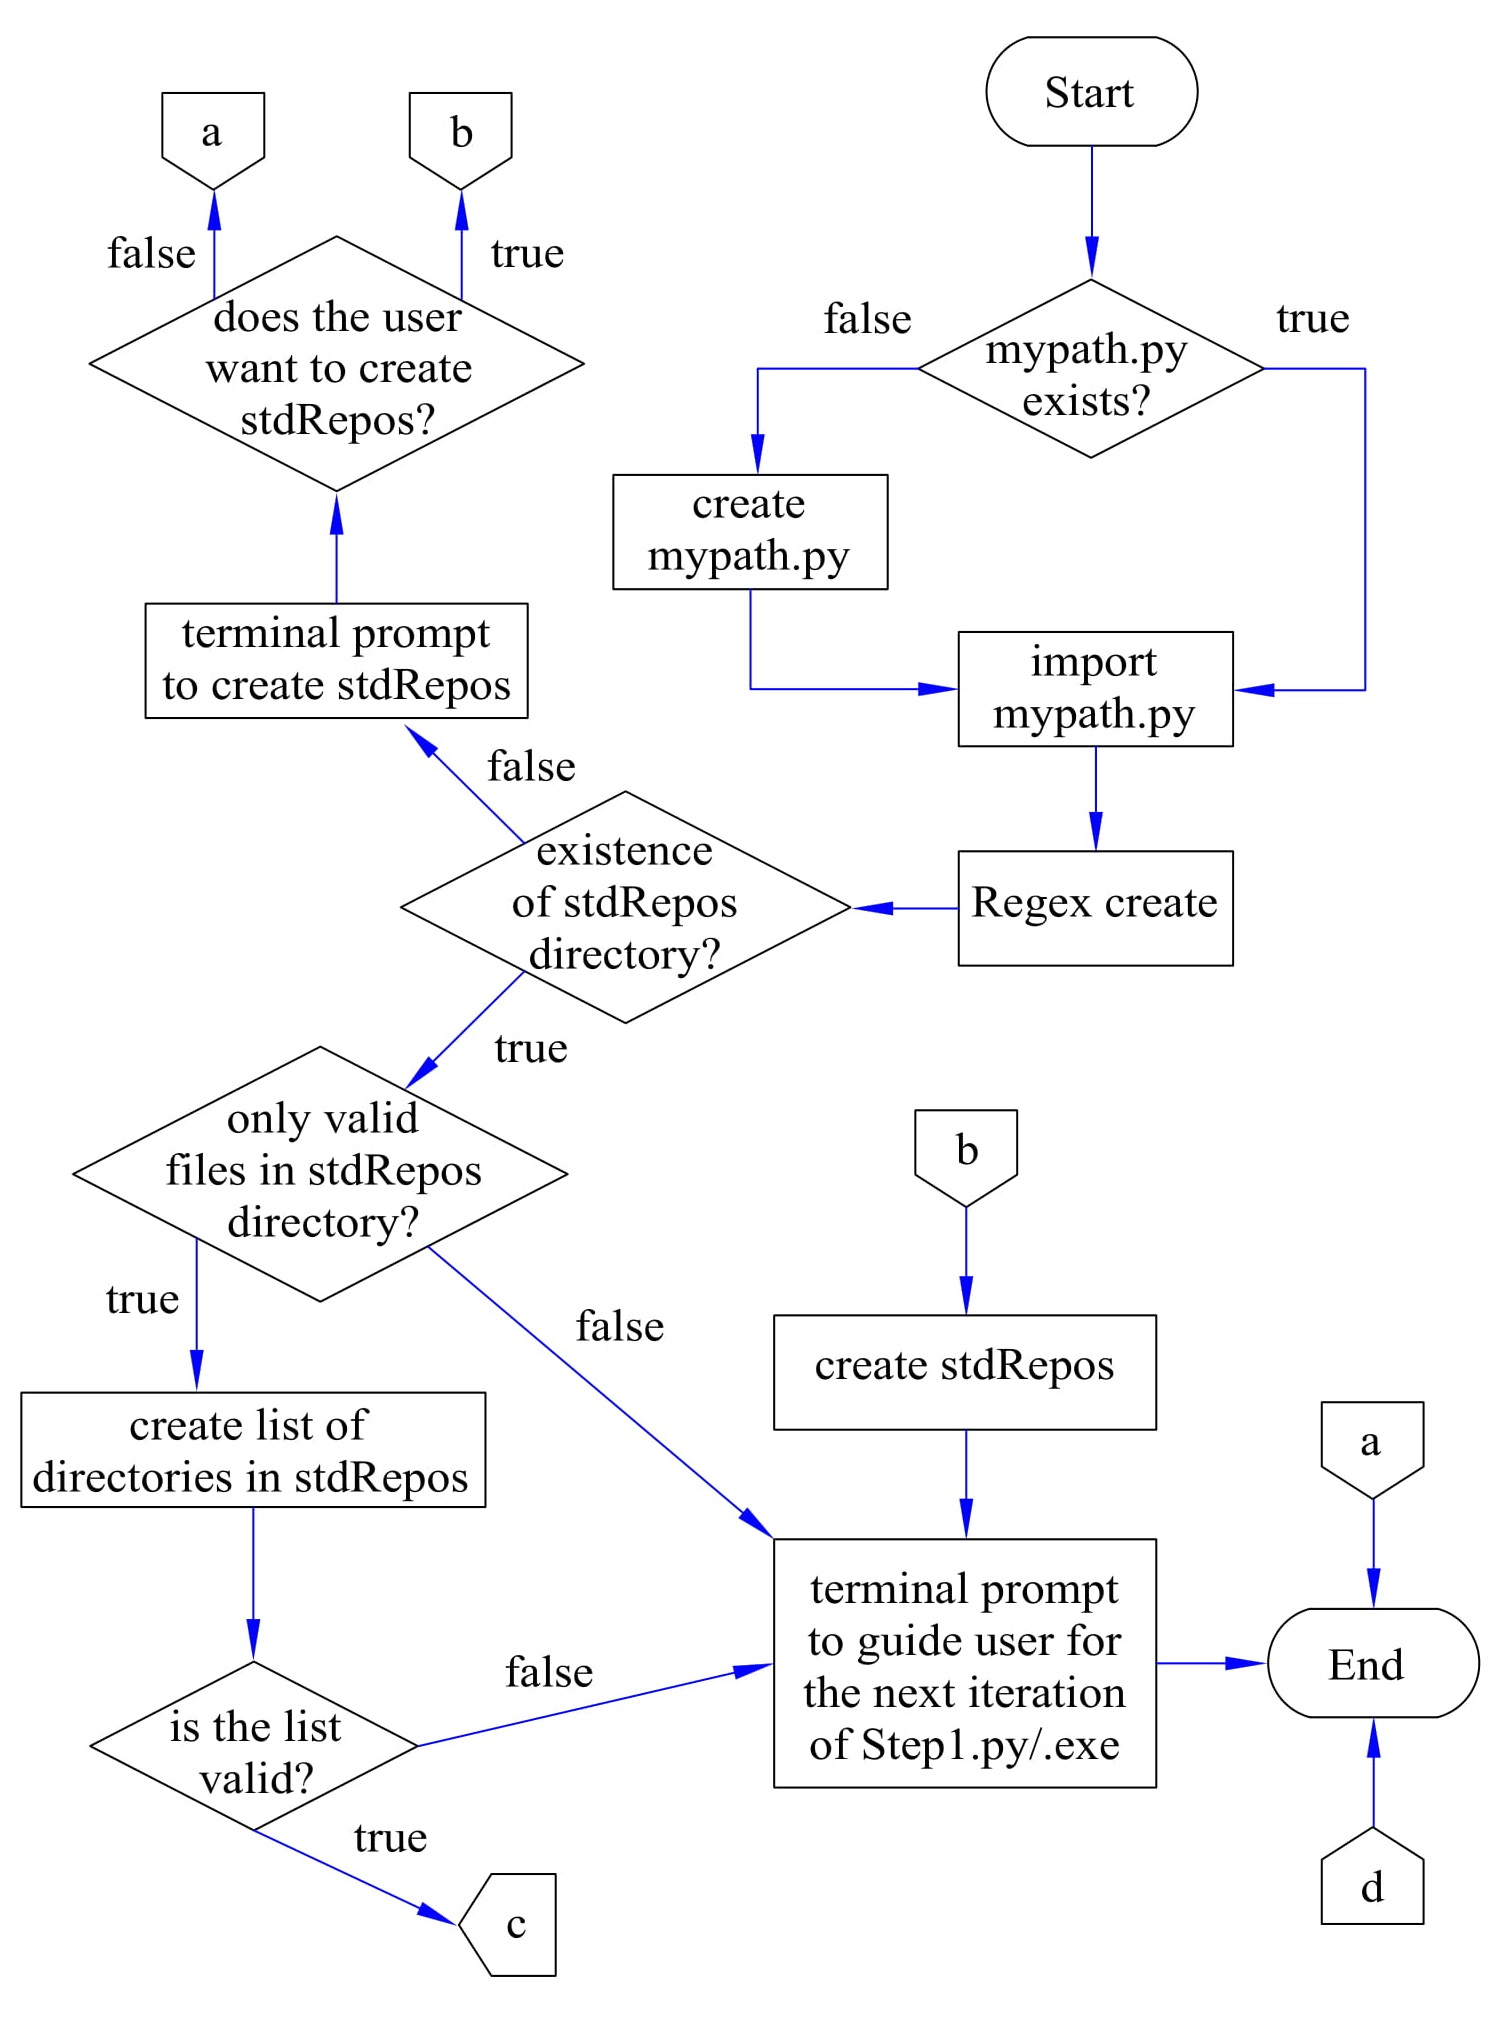
\includegraphics[width = 155mm]{1.1.jpg}
\caption{Step1 flow diagram 1}
\label{1.1}
\end{center}
\end{figure}

\begin{figure}[H]
\begin{center}
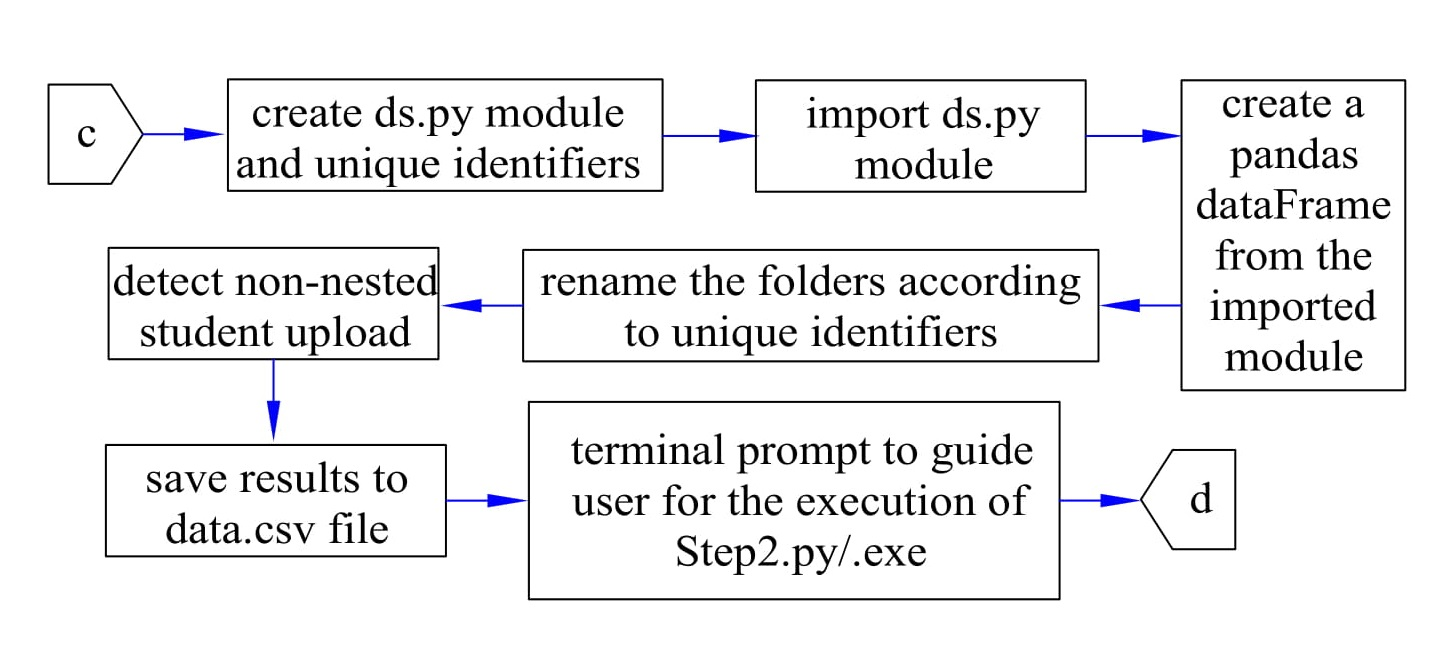
\includegraphics[width = 155mm]{1.2.jpg}
\caption{Step1 flow diagram 2}
\label{1.2}
\end{center}
\end{figure}

As can be see in Figure~\ref{1.1} and Figure~\ref{1.2}, the logical parts of the Step1.py/.exe are quite extensive and will only partially be discussed. 

\subsubsection{mypath.py module}
\label{mypath}

The various programs that comprise the autonomous system will be executed on a host PC other than the one they were created on. Since the user of the host PC can place the autonomous system (consisting of three programs) anywhere in the file system of the aforementioned PC, identifying the root repository becomes necessary. It is indeed important, that the programs in the autonomous chain, are able to execute regardless of where in the host file system they are located. 
\\\\
Regarding the above observation, it was decided that a python module is to be created in order to save the home, "stdRepos" and "data" directories. The code snippet below illustrates the process of creating the "data" directory as well as the mypath.py module. It further illustrates how the aforementioned module is imported into the program after creation.
\\\\
\lstinputlisting[label={code1},caption={mypath.py and data folder creation and import}, language=Python]{code1.py}

It can be seen from Listing~\ref{code1}: lines 13 - 24 that the program will create a "data" directory within the home directory (where the programs are located). In addition to the creation of this directory, a module is created and stored within the "data" directory, namely mypath.py \cite{Sweigart2015}.
\\\\
It is of note, that the aforementioned functionality strictly occurs if the "data" directory and the mypath.py module does not yet exist. If these entities do however exist, the module is simply imported as per  Listing~\ref{code1}: lines 5 - 11. Since Step1.py/.exe is created with multiple executions in mind, the decision was taken to use the above discussed approach.

\begin{figure}[H]
\begin{center}
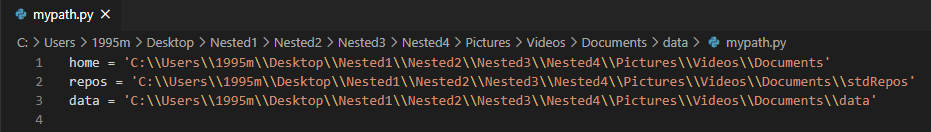
\includegraphics[width = 155mm]{mypath.pyCon.png}
\caption{mypath.py module content}
\label{mypath.pyCon}
\end{center}
\end{figure}

Figure~\ref{mypath.pyCon} illustrated the content of the pertaining module. Moreover, it illustrates how the directories of importance are stored regardless of location within a file system. The absolute path to the various directories are saved to be utilized by subsequent executions of Step1.py/.exe, in addition to the other programs in the autonomous chain.


\subsubsection{Regex creation}
\label{regex1}
As indicated in \textbf{\ref{p1} \nameref{p1}}, an important requisite of the autonomous process is the introduction of anonymity. It is, in fact, necessary to remove and replace all instances of student numbers from directory and file names for reasons mentioned in \textbf{\nameref{3}}. In order to facilitate the fulfilment of anonymity, it was decided to introduce regular expressions to the various programs in the autonomous system. These regular expressions are henceforth abbreviated simply as regex. 

\lstinputlisting[label={code2},caption={Regex initialization}, language=Python]{code2.py}

Listing~\ref{code2} depicts the regular expressions introduced as part of Step1.py/.exe. Lines 1-3 are simply regular expressions used to identify different variants of student numbers \cite{Sweigart2015}\cite{regex}. Line 4 consists of a regex pattern used to identify a valid student number unique identifier and will be expanded upon in \color{green}that part \color{black}.
\subsubsection{stdRepos directory}
\label{stdRepos}
\lstinputlisting[label={code3},caption={Regex initialization}, language=Python]{code3.py}

Listing~\ref{code3} depicts the code written to:
\\\\
\begin{enumerate}
\item Detect the existence of the "stdRepos" directory.
\item Create the "stdRepos" directory if the user so wishes.
\item Detect valid repositories within the "stdRepos" directory.
\item Create and handle all command prompts associated with the above mentioned functionality.
\end{enumerate}

It can be seen from Listing~\ref{code3}: Lines 1-21, that the program will test for the existence of the "stdRepos" folder within the home directory. If this directory is not detected, a command prompt will be displayed giving the user the option to create the "stdRepos" folder in the correct location. Thereafter, the program will exist after prompting the user to rerun Step1.py/.exe.
\\\\
It is assumed that the user will extract any student repositories within the "stdRepos" folder. It can be seen from Listing~\ref{code3}: Line 24, that the regex mentioned in \textbf{\ref{regex1} \nameref{regex1}}, is applied to the directory names within the "stdRepos" folder. If a match is detected a list is populated with the matched string. This list will be used in future functional blocks. 
\\\\
It can, lastly, be seen that any invalid files in the "stdRepos" folder will also be detected by the program. If indeed a folder/file is located within the directory but is not matched by a student number detection regex or a unique identifier regex, a command prompt will guide the user in the next step. The aforementioned functionality is depicted in Listing~\ref{code3}: Lines 27-40.

\subsubsection{ds.py module}
\label{ds}
\begin{figure}[H]
\begin{center}
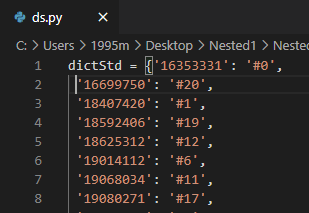
\includegraphics[width = 50mm]{ds.py.png}
\caption{ds.py module content}
\label{ds.pyCon}
\end{center}
\end{figure}

Figure~\ref{ds.pyCon} displays the content of the ds.py module. It depicts the linking of unique identifiers with student numbers. It is important to note that anonymity is not compromised by the ds.py module as it is deleted after the autonomous process finishes. Furthermore, each iteration of Step1.py/.exe randomly assigns unique identifiers to student numbers and the identifiers depicted in Figure~\ref{ds.pyCon}, will change from iteration to iteration. 

\lstinputlisting[label={code4},caption={ds.py creation}, language=Python]{code4.py}

Listing~\ref{code4}: Lines 1-12 depicts the code written to create a dictionary based on the content of the "stdRepos" folder. Randomly produce indexes are linked to student numbers and stored in a dictionary. It furthermore, illustrates (lines 14-24) how the mentioned dictionary is stored as a python module to be imported and utilized by the other steps in the autonomous process. 

\subsubsection{Pandas DataFrame}
\label{datFra}
It was decided to use a Pandas Data Frame to store any information extracted from student repositories. A Pandas Data Frame was selected above similar frameworks due to the ease with which data in the frame can be manipulated and searched. In order to populate the Pandas Data Frame, the previously created ds.py module must be imported by the program. This is all done in a very straight forward and standard way and will thus not be expanded upon.  


\subsubsection{Rename the folders}
\label{renFol}
\lstinputlisting[label={code5},caption={Folder renaming}, language=Python]{code5.py}

In Listing~\ref{code5}: lines 1-12, it can be observed that the folders within the "stdRepos" directory are renamed using a nested for-loop. The first for-loop iterates through all the folders within the "stdRepos" directory. The second (nested) for-loop, loops through the Pandas Data Frame (populated with unique identifiers linked to student numbers) and renames the current folder (the subject of the first for-loop) to the linked unique identifier.
\\\\
In short, for each folder in the "stdRepos" directory the Pandas Data Frame is looped to find the specific unique identifier associated with the pertaining folder student number. The folders are then renamed according to the identifier. 


\subsubsection{data.csv file}
\label{data.csv}
Lastly, the previously mentioned Pandas Data Frame is stored as data.csv in the "data" directory. This file (data.csv) will be used to facilitate the population of Pandas Data Frames used by the subsequent steps in the automation process. 



\subsection{Step2.py}
\label{step2}

\begin{figure}[H]
\begin{center}
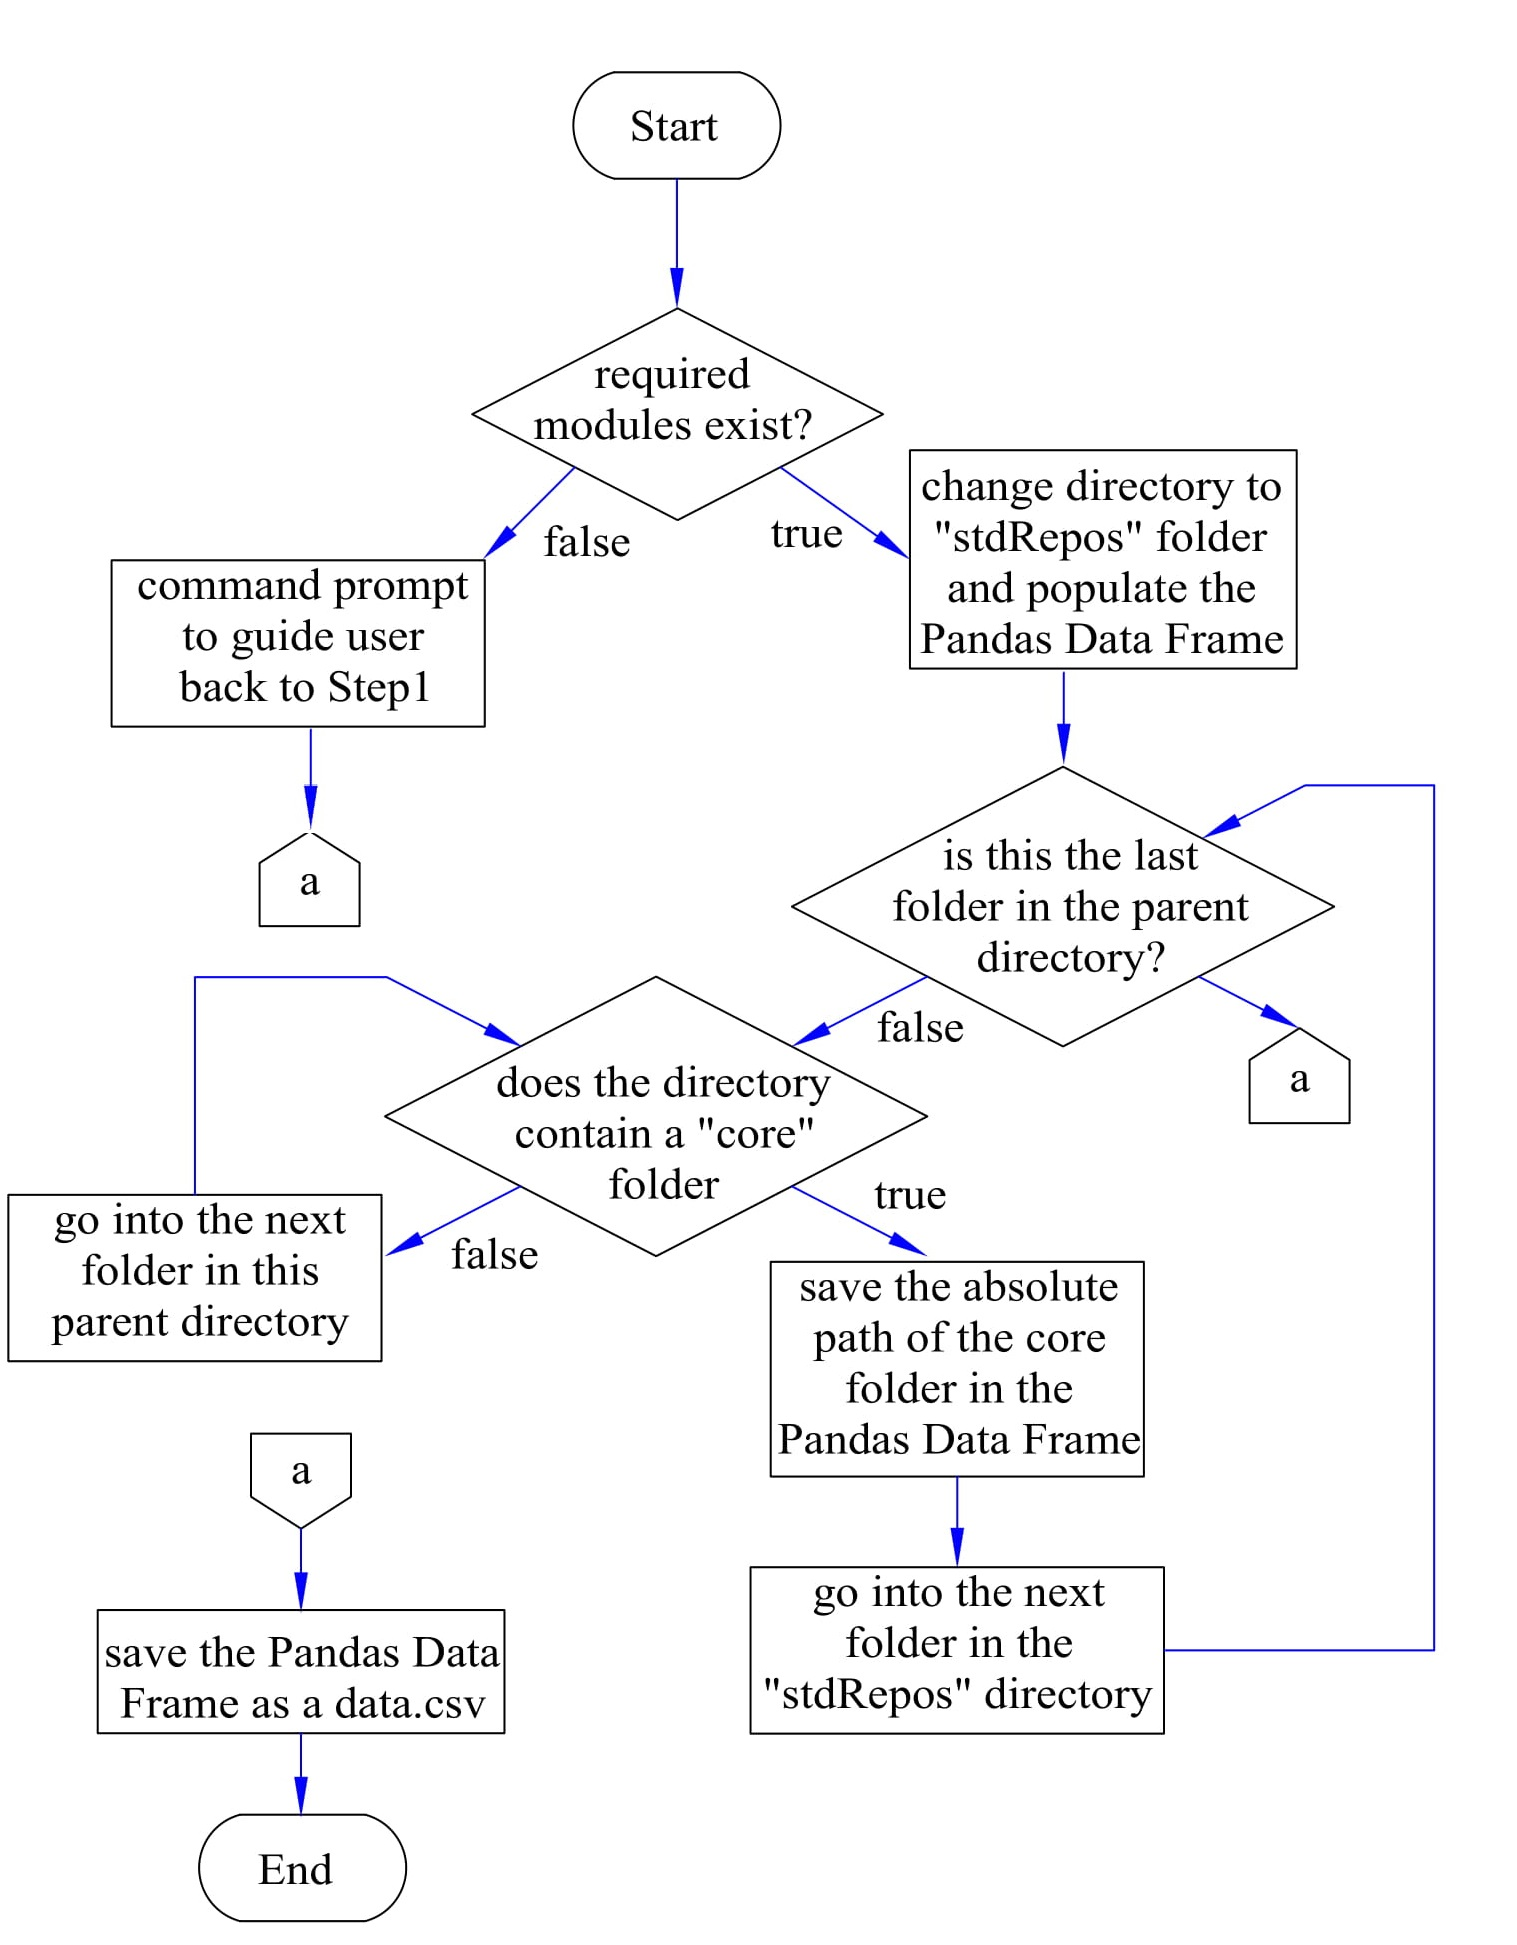
\includegraphics[width = 155mm]{2.jpg}
\caption{Step2 flow diagram}
\label{2}
\end{center}
\end{figure}

\subsection{Step3.py}
\label{step3}

\section{Windows executable files}
\label{exe}
